% Standalone write-up for the `fbl` library: theory, method, and all results.
% Self-contained (standard packages only; no thesis macros).
% Build:  pdflatex writeup.tex   (run from docs/; figures are ../examples/figures + .)
\documentclass[11pt]{article}
\usepackage[margin=1in]{geometry}
\usepackage{amsmath,amssymb}
\usepackage{graphicx}
\usepackage{booktabs}
\usepackage{subcaption}
\usepackage{float}
\usepackage[hidelinks]{hyperref}
\graphicspath{{../examples/figures/}{./}}

\newcommand{\Phib}{\Phi}
\newcommand{\Tr}{^{\!\top}}
\title{\textbf{Finite-Blocklength Bounds with Prior Optimization:\\ the $\Phi$-view}}
\author{Nir Elkayam \\ \small the \texttt{fbl} library}
\date{}

\begin{document}
\maketitle

\begin{abstract}
\noindent
\texttt{fbl} is a validated library for one-shot / finite-blocklength information
theory built on the pairwise-error-probability (PEP) error-spectrum framework. It
covers channel coding, rate--distortion (average and excess), and joint
source--channel coding (JSCC), in two flavours (exact one-shot / method-of-types).
Its distinguishing feature is the \emph{achievability} prior optimization, which we
show is a single \emph{convex program} on the simplex,
$\max_Q\, c\Tr \Phi(AQ)$, where the kernel of the bound chooses the fixed potential
$\Phi$. We solve it directly by a first-order \emph{simplex march} that is exact for
any kernel and certifies its own optimality by a water-filling (KKT) condition; the
classical exact convex solvers (a quadratic program for the $\mathrm{RCU}^+$ kernel,
a bracketing LP otherwise) are special cases retained as validation anchors. We
report a self-contained figure suite for four pinned use cases, all numbers backed
by a $107$-test cross-check suite.
\end{abstract}

\section{Introduction}
For each setting the library computes three quantities: the \emph{achievable}
(random-coding) bound, the \emph{converse} (meta-converse LP), and---one-shot
only---a \emph{Monte-Carlo} realization. The converse optimizes the prior
point-wise (a linear program at one threshold). The achievability bound is a kernel
integral of the \emph{whole} error spectrum, so its prior optimization is global. We
show it is nonetheless a convex program with a common form, and that the optimal
prior can be found exactly and certified intrinsically. The practical question the
suite answers is then sharp: \emph{given the certified optimal prior, how large is
the gap to a memoryless prior?}

\section{The unified $\Phi$-view}\label{sec:phi}
Fix an output $y$ and a metric $m(x,y)\ge0$. Under the dithered tie rule the PEP of a
candidate drawn from the prior $Q_X$ is uniform on $[0,1]$, so the value-weighted
spectrum and its average against a non-negative kernel $\kappa$ are
\begin{equation}
F(w\mid y)=\mathbb{E}_{X\sim Q_X}\!\big[m(X,y)\,\mathbf{1}\{\mathrm{PEP}\le w\}\big],
\qquad J=\int_0^1 F(w\mid y)\,\kappa(w)\,\mathrm{d}w .
\end{equation}
The prior enters through one linear map---the cumulative-rank profile
$(AQ_X)(\nu)=Q_X\{x: m(x,y)\ge\nu\}$---and the value through the functional
$c\Tr v=\int_0^\infty v(\nu)\,\mathrm{d}\nu$. With the kernel potential
$\Phi_\kappa(\sigma)=\int_0^1\min\{w,\sigma\}\,\kappa(w)\,\mathrm{d}w$ one has the
\emph{nonlinear program of the PEP},
\begin{equation}\label{eq:nlp}
\boxed{\,J(Q_X)=c\Tr \Phi_\kappa(AQ_X)\,}\qquad
\text{finite alphabet: } J=\sum_j c_j\,\Phi_\kappa(\sigma_j),
\end{equation}
with $\sigma_j$ the cumulative masses (sorted by metric) and $c_j$ the value-gaps.
The potential satisfies $\Phi_\kappa(0)=0$, $\Phi_\kappa'(\sigma)=\int_\sigma^1\kappa\ge0$,
$\Phi_\kappa''=-\kappa$, so $\Phi_\kappa$ is concave; since $AQ_X$ is linear and
$c\ge0$ in the matched case, $J$ is \textbf{concave in $Q_X$} and prior optimization
is a convex program over the simplex. Two tails occur: the \emph{error} tail
(channel/JSCC) maximizes a concave $J$; the \emph{correct} tail (rate--distortion)
minimizes a convex $J$ in the dual (CDF) variable.

\paragraph{The kernel chooses the program.}
Table~\ref{tab:phi} lists the potentials. The converse is the point-mass kernel
$\kappa=\delta_{w_0}$, whose ramp potential is piecewise-linear (an LP). The
$\mathrm{RCU}^+$ potential is a clamped parabola---\emph{quadratic}---so its convex
program is a quadratic program (QP). The exact-RC and rate--distortion potentials are
non-polynomial, handled either by a bracketing LP (secant/tangent of $\Phi$) or
exactly by the march below.

\begin{table}[H]\centering
\begin{tabular}{@{}llll@{}}
\toprule
bound & potential $\Phi_\kappa$ & shape & program \\
\midrule
converse, level $w_0$ & $\min\{\sigma,w_0\}$ & piecewise-linear & LP \\
channel, $\mathrm{RCU}^+$ & $\sigma-\tfrac{M-1}{2}\sigma^2$ (clamped) & quadratic & QP \\
channel, exact & $\tfrac1M\big(1-(1-\sigma)^M\big)$ & concave & bracket / march \\
rate--distortion, exact & $(1-\tau)^M$ & convex & bracket / march \\
rate--distortion, smooth & $e^{-M\tau}$ & convex & bracket / march \\
\bottomrule
\end{tabular}
\caption{The potentials instantiating~\eqref{eq:nlp} ($M$ the codebook size). The
QP is simply the case of a \emph{quadratic} $\Phi$.}
\label{tab:phi}
\end{table}

\paragraph{The simplex march and its certificate.}
We maximize $f=\mathrm{sense}\cdot J$ ($\mathrm{sense}=+1$ channel/JSCC, $-1$ RD)
directly on the simplex by projected gradient / Frank--Wolfe, using the analytic
water-fill gradient
\begin{equation}
\nabla f(Q)=A\Tr\!\big(c\odot \Phi'(AQ)\big),\qquad
g(x)=\sum_y\sum_{i\ \text{fed by}\ x}\!\mathrm{ratio}_i\!\sum_{j\ge i} c_j\,\Phi'(\sigma_j).
\end{equation}
The prior obeys a \emph{product} of simplices (one global simplex for channel/RD; one
per source-type block for JSCC). Optimality is the \textbf{water-filling KKT
condition}---$\nabla f$ flat on the support and dominated off it, per block---and the
Frank--Wolfe gap $g(Q)=\sum_b\big(\max_b\nabla f-\langle\nabla f_b,Q_b\rangle\big)$
is a rigorous suboptimality certificate, $0\le f(Q^\star)-f(Q)\le g(Q)$. Thus the
achieved bound is always valid (a feasible prior), and $g(Q)$ brackets the
prior-optimized optimum without any second solver. The march is exact for every
kernel; the QP/bracketing-LP are cvxpy instantiations of the \emph{same} program,
kept as independent machine-precision anchors.

\section{The library}\label{sec:lib}
The code is a small dependency DAG (infra $\to$ engines $\to$ prior-opt $\to$
examples). The prior-opt layer is \texttt{phi\_view} (the relaxation
$J=c\Tr\Phi(AQ)$, its potentials and evaluators) and \texttt{phi\_simplex} (the
march and the \texttt{check\_kkt} certificate); the exact convex solvers remain as
anchors.

\begin{figure}[H]\centering
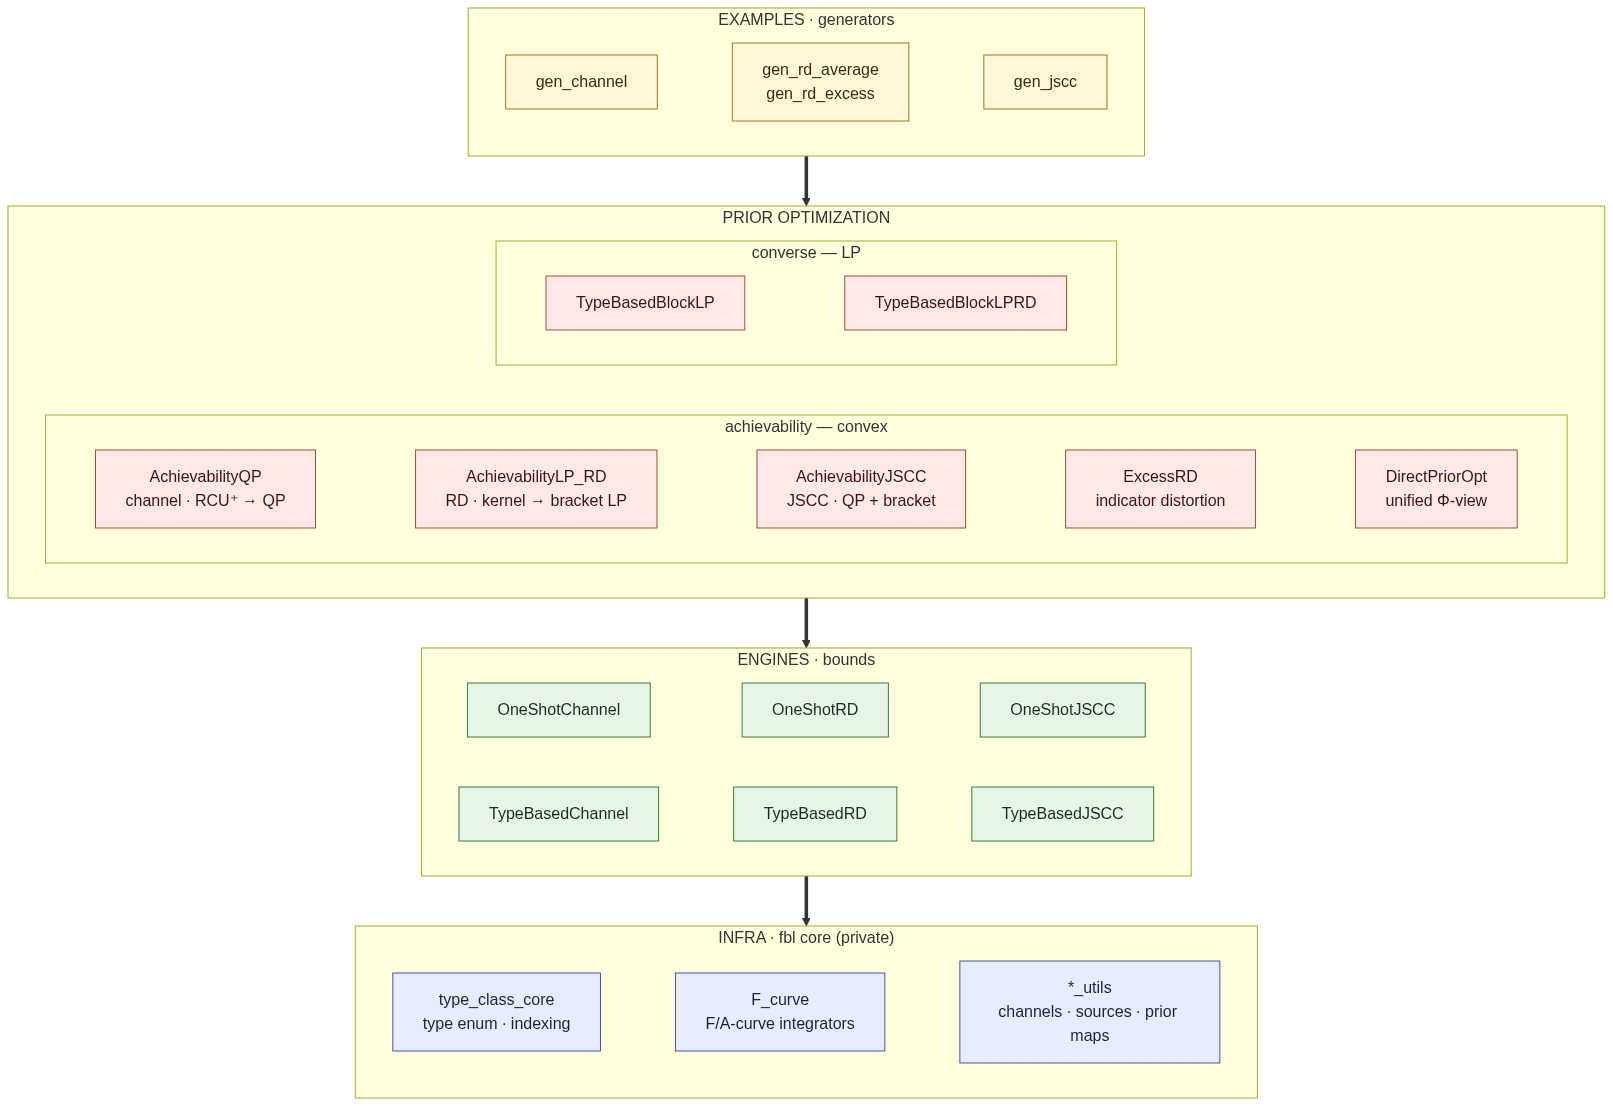
\includegraphics[width=0.86\textwidth]{architecture.png}
\caption{Module dependency DAG. Prior optimization is the $\Phi$-view mechanism
(\texttt{phi\_view}/\texttt{phi\_simplex}) with the exact solvers as anchors.}
\end{figure}
\begin{figure}[H]\centering
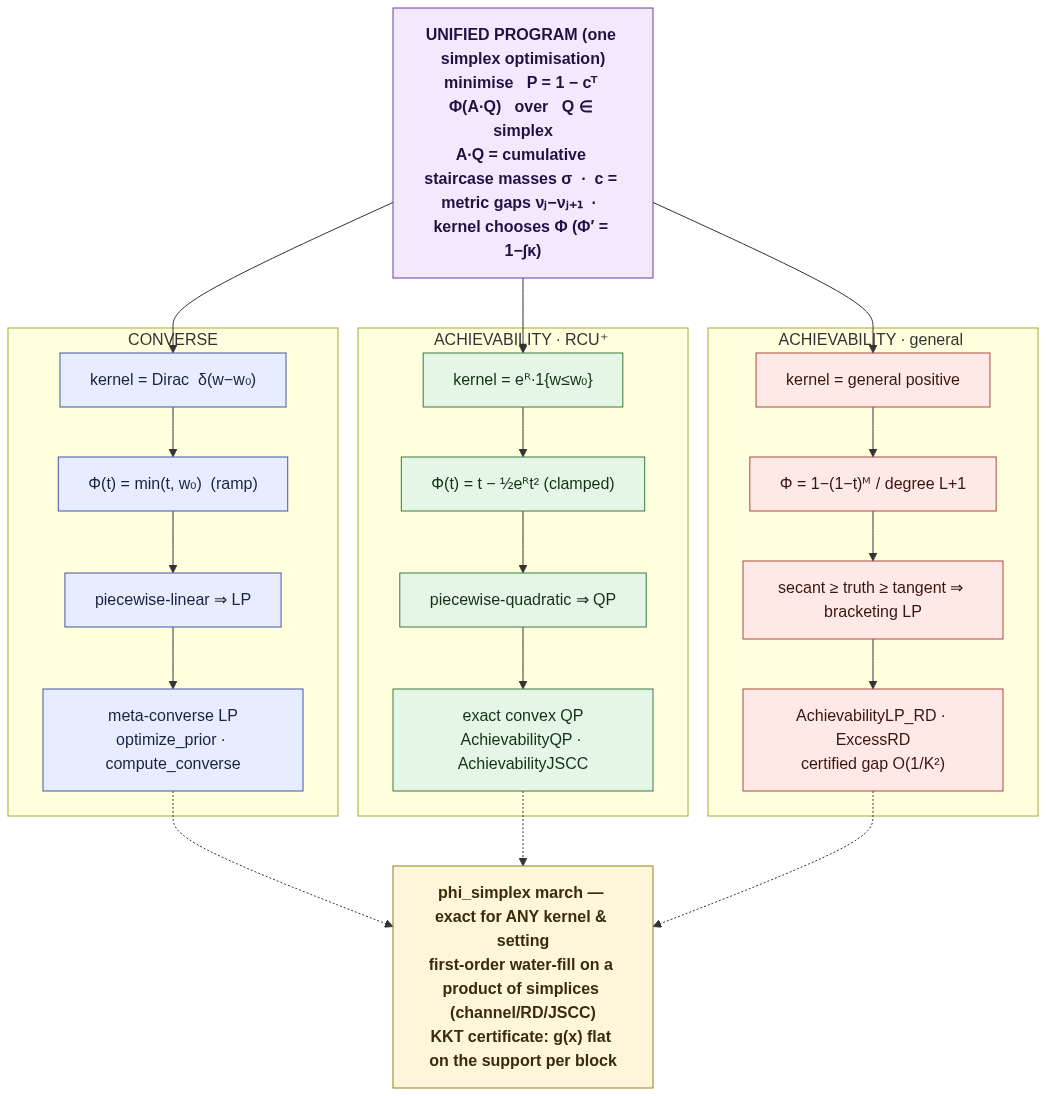
\includegraphics[width=0.92\textwidth]{algorithms.png}
\caption{The unified program: the kernel selects $\Phi$ (Dirac$\to$LP,
$\mathrm{RCU}^+\to$QP, general$\to$bracket), and the simplex march solves all of
them exactly.}
\end{figure}

\paragraph{Validation.} No closed-form oracle exists, so every quantity is
cross-checked ($107$ tests): one-shot $\leftrightarrow$ type-based at small $n$;
RCU expectation $\leftrightarrow$ Monte-Carlo; converse $\le$ achievable; the
$\Phi$-view identity $J=c\Tr\Phi(AQ)$ against an independent computation in both
representations and all settings; and the march optimum against the exact solvers
\emph{and} the intrinsic KKT certificate (rejected off the optimum).

\section{Results}\label{sec:results}
Each use case is pinned to a single channel/source. \textbf{G1} validates the bound
against Monte-Carlo at small $n$; \textbf{G2} is the prior gap (optimal achievable
prior vs.\ optimal memoryless vs.\ the two marginal-memoryless priors); \textbf{G3}
compares exact random coding to a closed-form surrogate; \textbf{G4} contrasts the
error/distortion spectra of the converse- and achievability-optimal priors; and
\textbf{G5} replaces each optimal prior by its i.i.d.\ \emph{product} (marginalized)
version and shows how the achievable bound changes. The achievability-optimal prior
is the KKT-certified march; the bound is the exact random-coding kernel. G1 stays at
$n=8$; G2--G5 are shown at $n=8$ and $n=20$.

\subsection{Channel coding --- $Z(0.1)$}
The non-product prior gain peaks at low rate and grows with $n$
($\approx2.0\%$ at $n=8$, $\approx3.3\%$ at $n=20$). The converse-optimal prior,
reused for achievability, is $5\times$ worse at $n=8$ and $15\times$ at $n=20$.
\begin{figure}[H]\centering
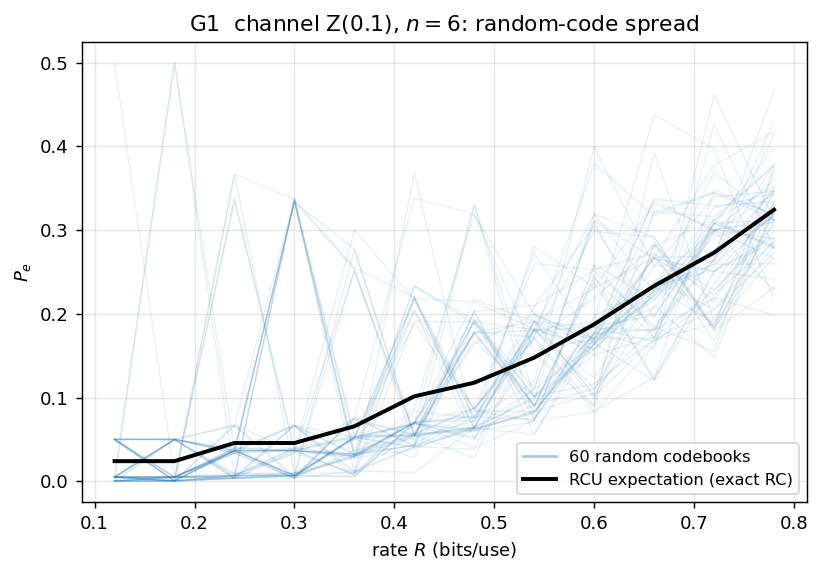
\includegraphics[width=0.62\textwidth]{channel_g1_mc_spread.png}
\caption{G1 ($n=8$): random-coding expectation vs.\ $60$ Monte-Carlo codebooks.}
\end{figure}
\begin{figure}[H]\centering
\begin{subfigure}{0.49\textwidth}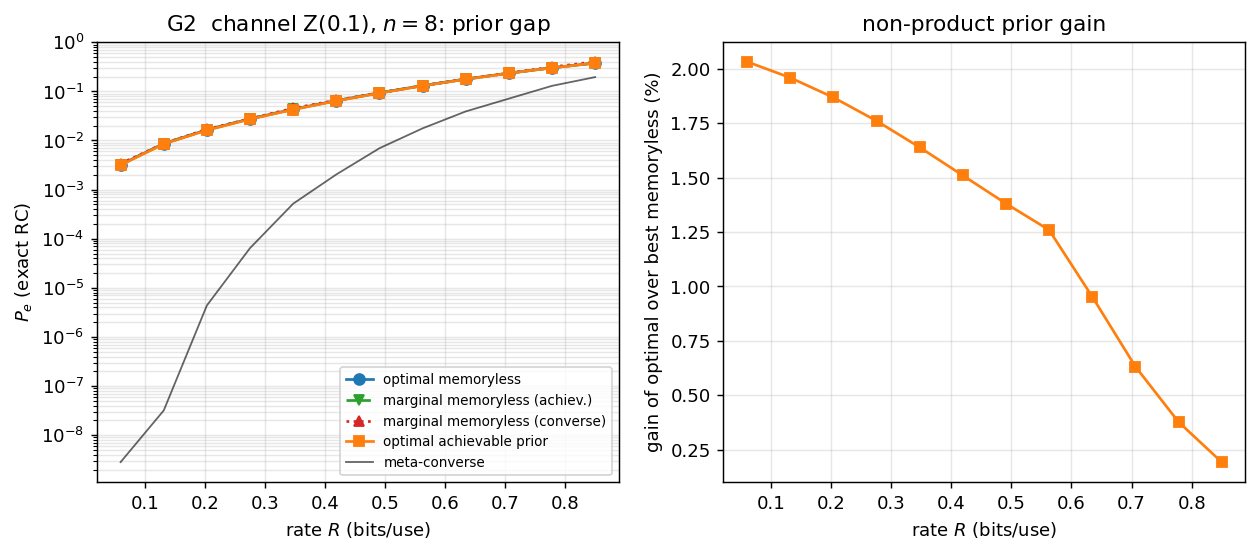
\includegraphics[width=\linewidth]{channel_g2_prior_gap_n8.png}\caption{$n=8$}\end{subfigure}\hfill
\begin{subfigure}{0.49\textwidth}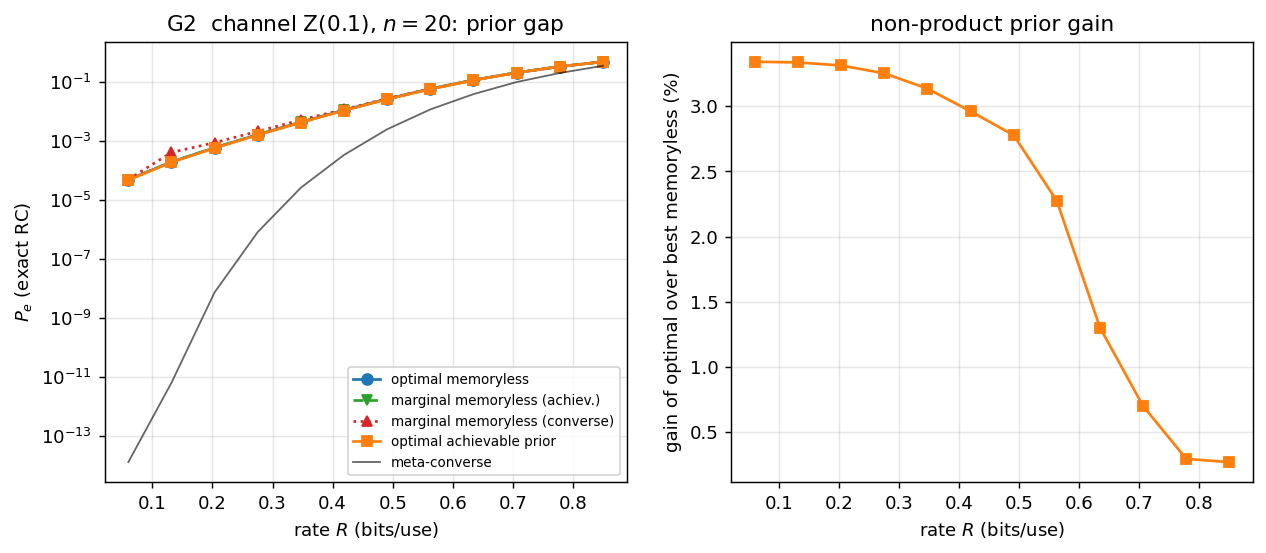
\includegraphics[width=\linewidth]{channel_g2_prior_gap_n20.png}\caption{$n=20$}\end{subfigure}
\caption{G2 --- the prior gap (exact kernel). Right panels: gain of the optimal
prior over the best memoryless prior.}
\end{figure}
\begin{figure}[H]\centering
\begin{subfigure}{0.49\textwidth}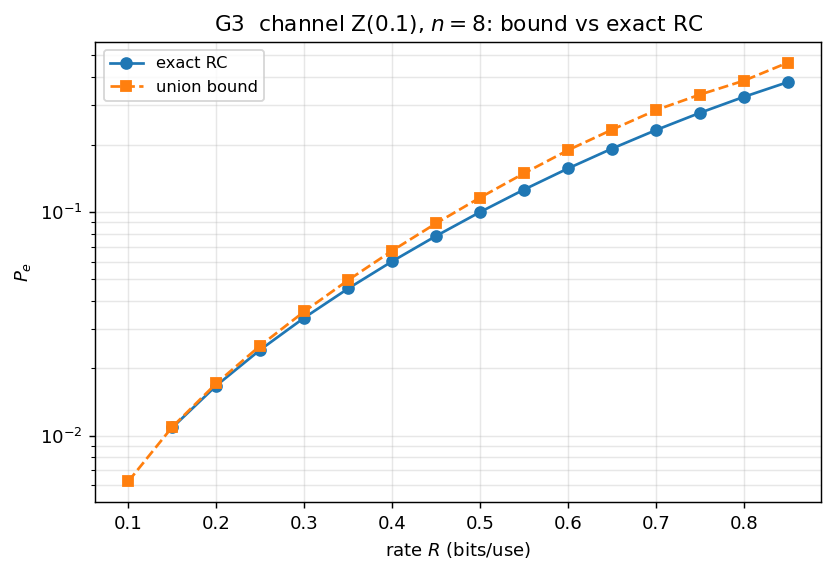
\includegraphics[width=\linewidth]{channel_g3_bounds_vs_exact_n8.png}\caption{$n=8$}\end{subfigure}\hfill
\begin{subfigure}{0.49\textwidth}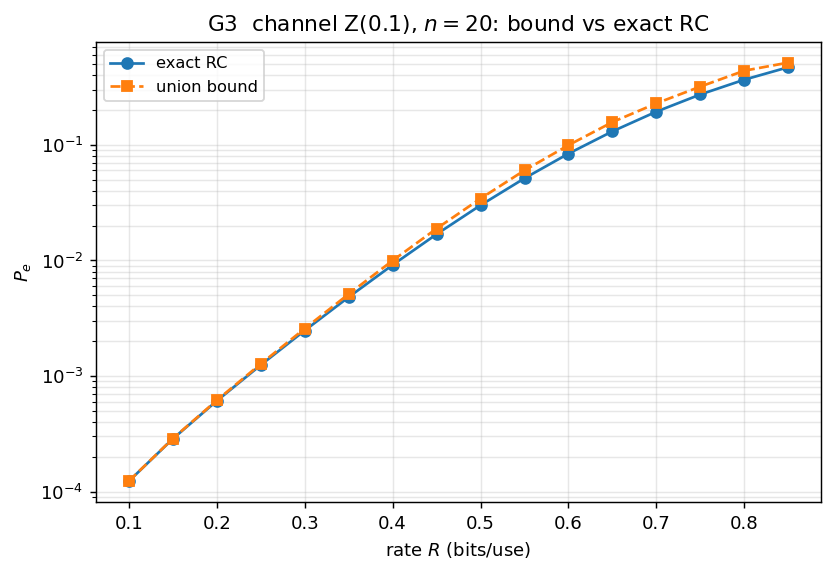
\includegraphics[width=\linewidth]{channel_g3_bounds_vs_exact_n20.png}\caption{$n=20$}\end{subfigure}
\caption{G3 --- exact random coding vs.\ the union bound.}
\end{figure}
\begin{figure}[H]\centering
\begin{subfigure}{0.49\textwidth}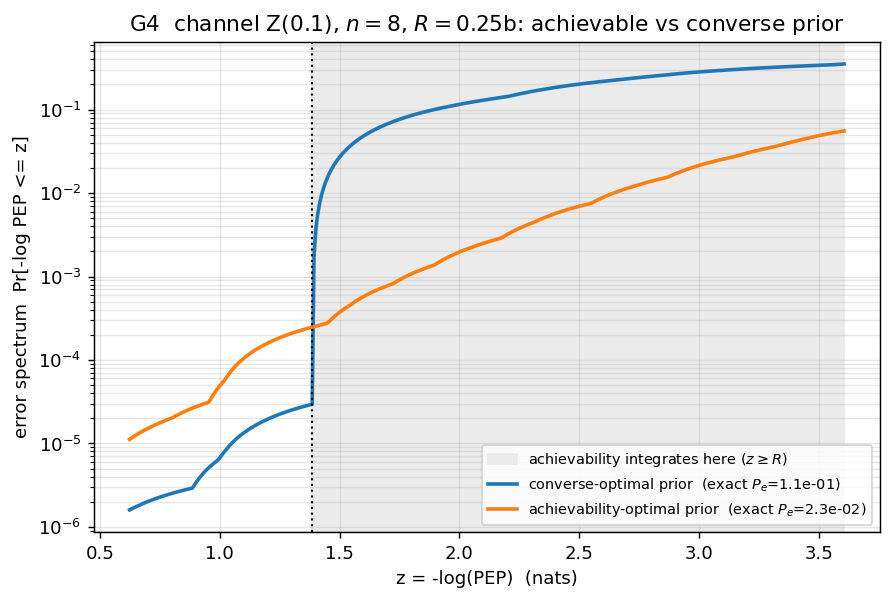
\includegraphics[width=\linewidth]{channel_g4_fcurve_compare_n8.png}\caption{$n=8$}\end{subfigure}\hfill
\begin{subfigure}{0.49\textwidth}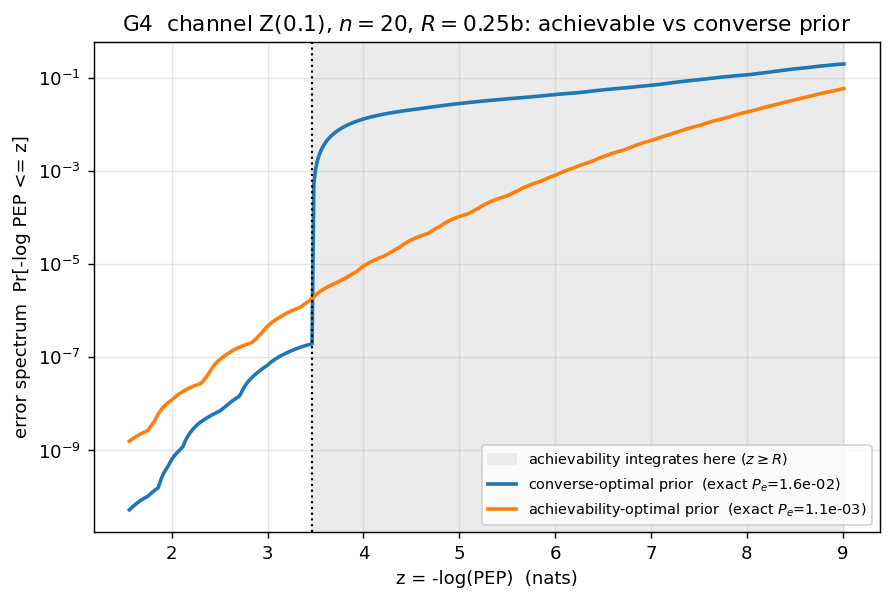
\includegraphics[width=\linewidth]{channel_g4_fcurve_compare_n20.png}\caption{$n=20$}\end{subfigure}
\caption{G4 --- error spectrum of the achievability- vs.\ converse-optimal prior.}
\end{figure}
\begin{figure}[H]\centering
\begin{subfigure}{0.49\textwidth}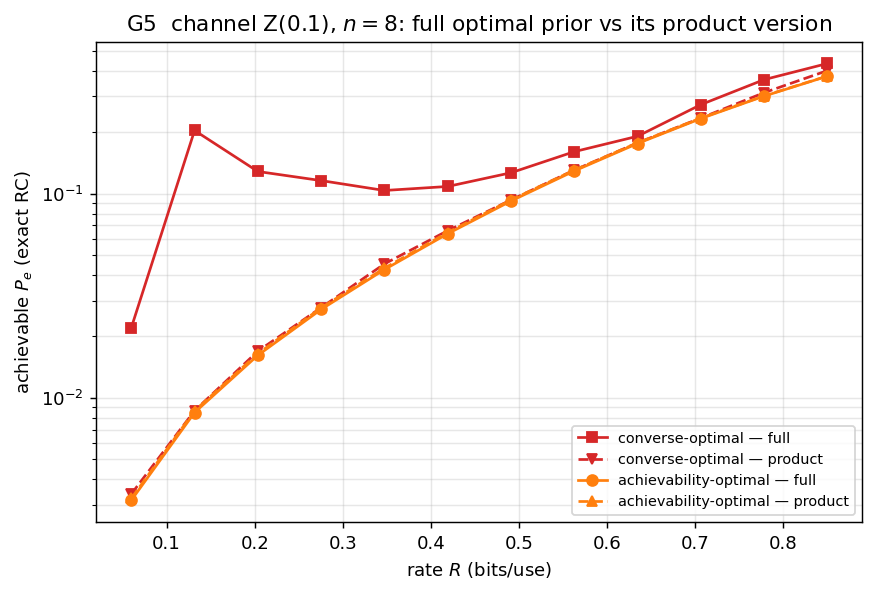
\includegraphics[width=\linewidth]{channel_g5_full_vs_product_n8.png}\caption{$n=8$}\end{subfigure}\hfill
\begin{subfigure}{0.49\textwidth}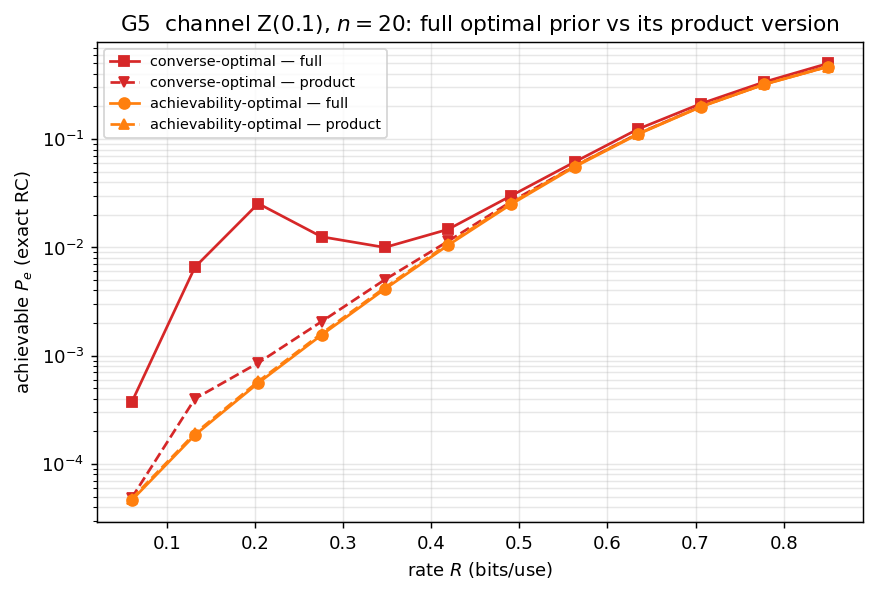
\includegraphics[width=\linewidth]{channel_g5_full_vs_product_n20.png}\caption{$n=20$}\end{subfigure}
\caption{G5 --- each optimal prior vs.\ its i.i.d.\ \emph{product} (marginalized)
version. The converse-optimal prior (red, full) is poor for achievability but its
product collapses onto the optimum; the achievability-optimal prior is unchanged.}
\end{figure}

\subsection{Rate--distortion, average --- BMS$(0.25)$ + Hamming}
The gain over the best memoryless prior is $\approx5.4\%$ ($n=8$) / $5.9\%$
($n=20$); the converse and achievability priors are nearly identical
($D:0.1551\!\to\!0.1529$ at $n=8$).
\begin{figure}[H]\centering
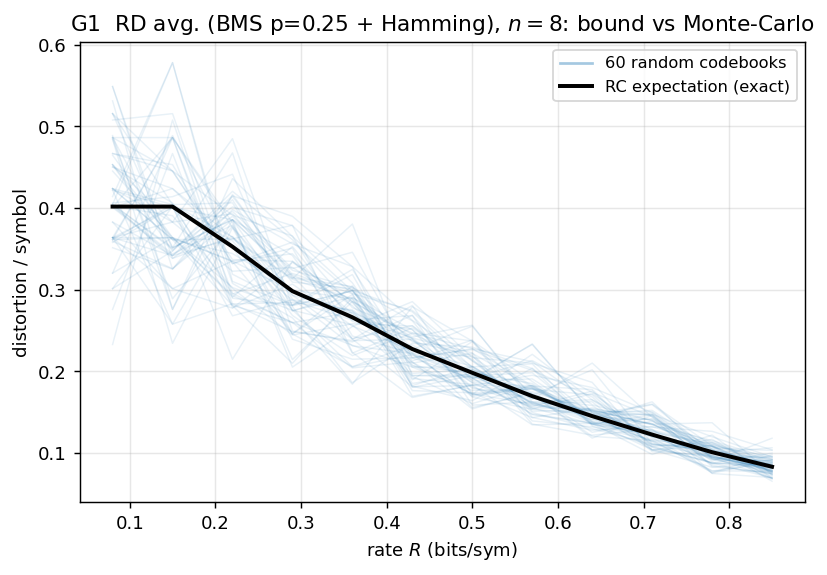
\includegraphics[width=0.62\textwidth]{rd_avg_g1_mc_spread.png}
\caption{G1 ($n=8$): realized distortion vs.\ the random-coding expectation.}
\end{figure}
\begin{figure}[H]\centering
\begin{subfigure}{0.49\textwidth}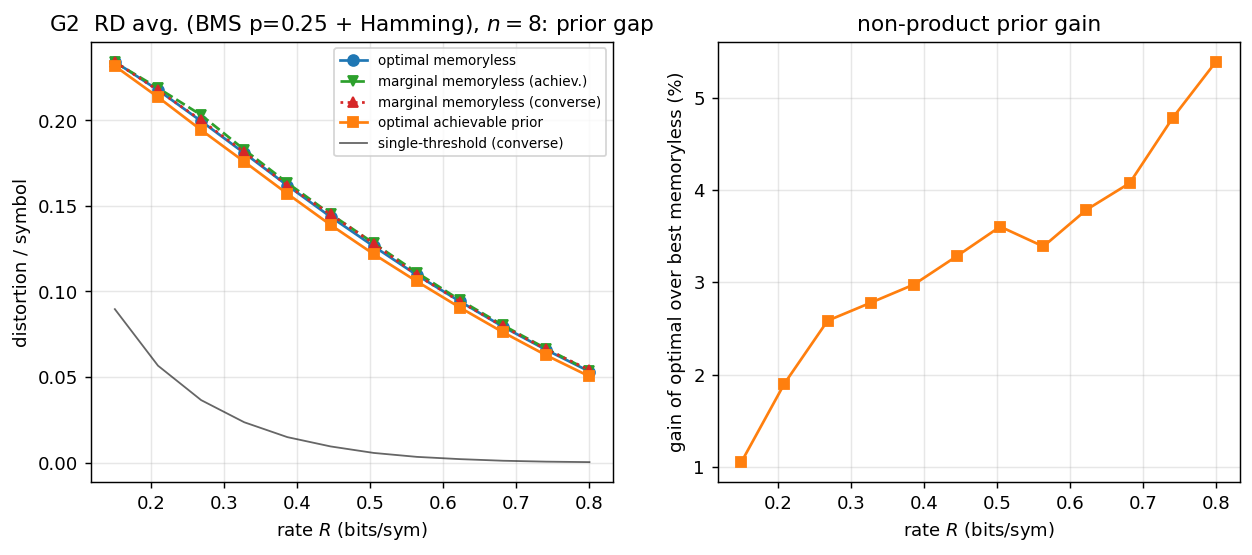
\includegraphics[width=\linewidth]{rd_avg_g2_prior_gap_n8.png}\caption{$n=8$}\end{subfigure}\hfill
\begin{subfigure}{0.49\textwidth}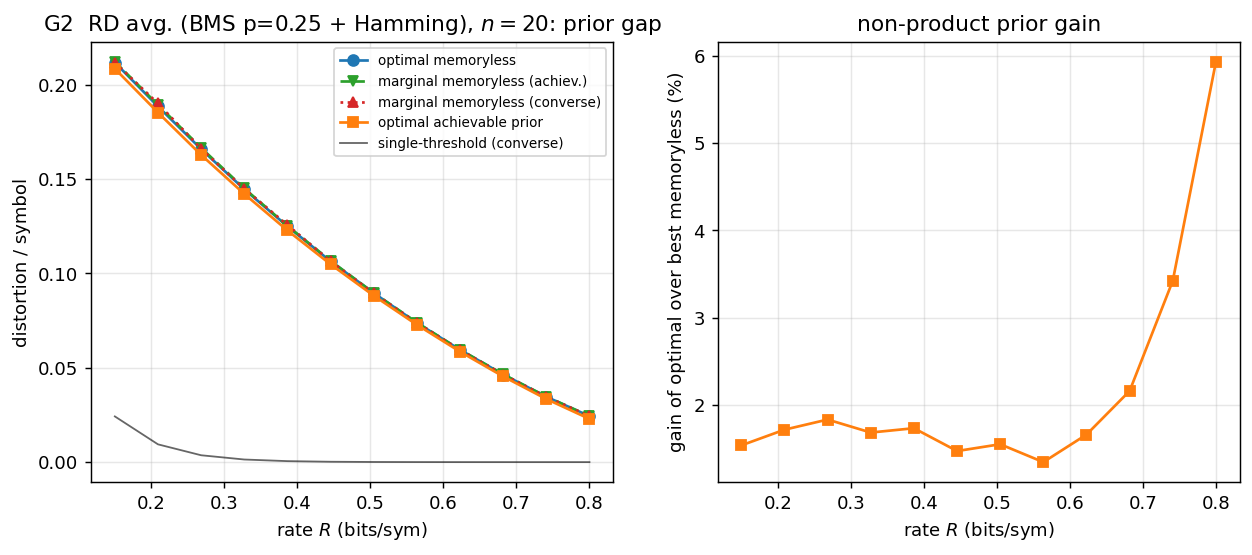
\includegraphics[width=\linewidth]{rd_avg_g2_prior_gap_n20.png}\caption{$n=20$}\end{subfigure}
\caption{G2 --- prior gap (exact best-of-$M$ kernel).}
\end{figure}
\begin{figure}[H]\centering
\begin{subfigure}{0.49\textwidth}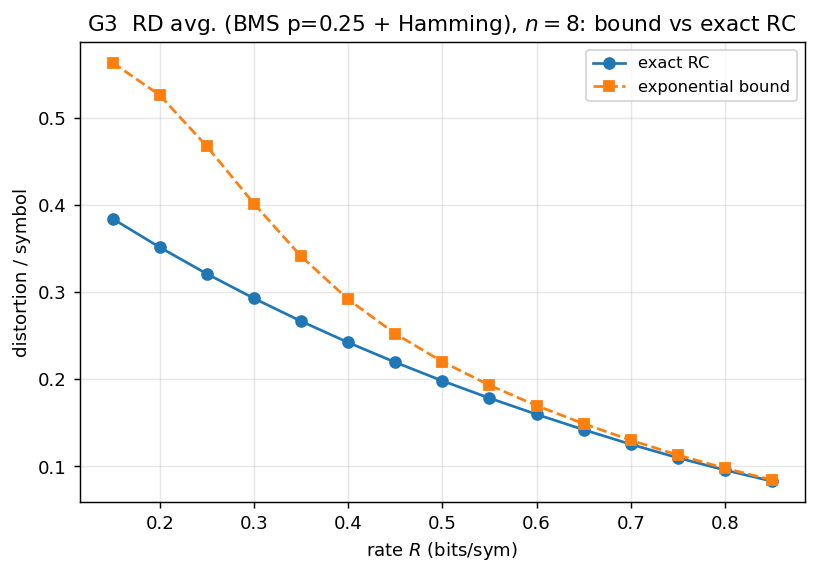
\includegraphics[width=\linewidth]{rd_avg_g3_bounds_vs_exact_n8.png}\caption{$n=8$}\end{subfigure}\hfill
\begin{subfigure}{0.49\textwidth}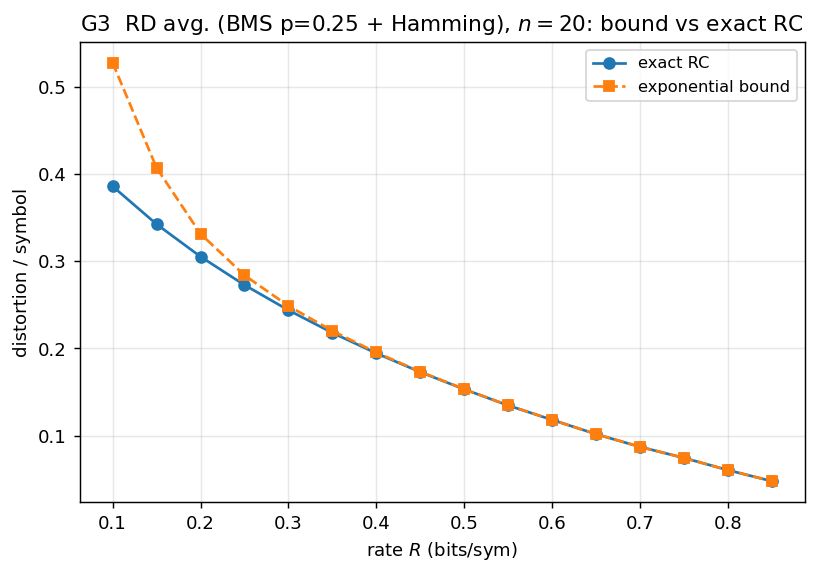
\includegraphics[width=\linewidth]{rd_avg_g3_bounds_vs_exact_n20.png}\caption{$n=20$}\end{subfigure}
\caption{G3 --- exact random coding vs.\ the exponential surrogate.}
\end{figure}
\begin{figure}[H]\centering
\begin{subfigure}{0.49\textwidth}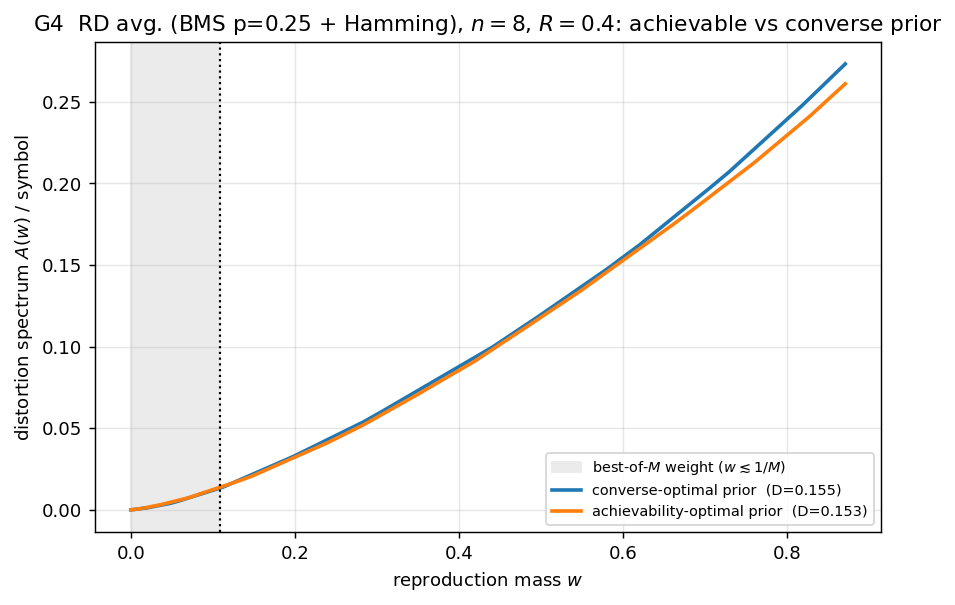
\includegraphics[width=\linewidth]{rd_avg_g4_fcurve_compare_n8.png}\caption{$n=8$}\end{subfigure}\hfill
\begin{subfigure}{0.49\textwidth}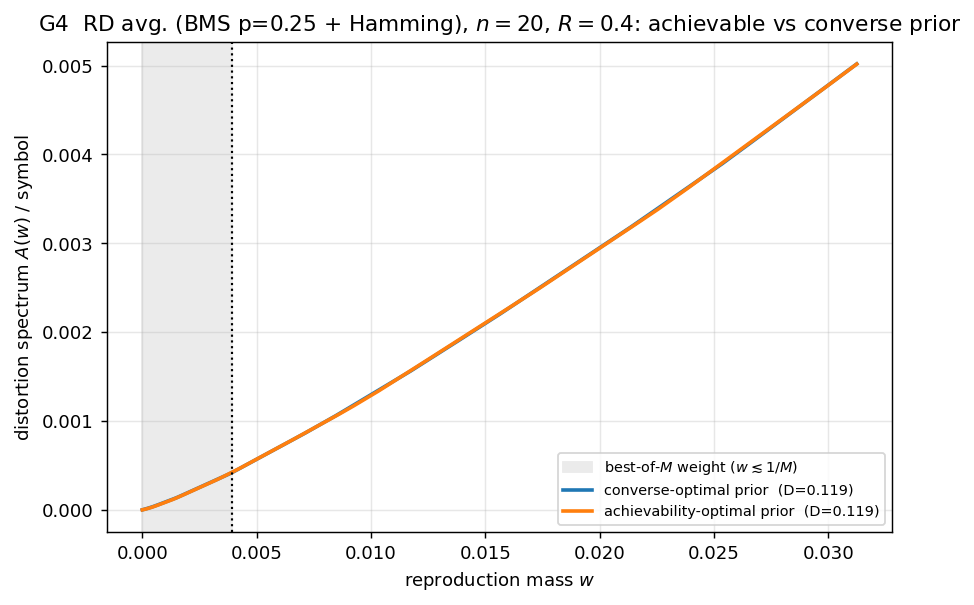
\includegraphics[width=\linewidth]{rd_avg_g4_fcurve_compare_n20.png}\caption{$n=20$}\end{subfigure}
\caption{G4 --- distortion spectra (nearly identical priors).}
\end{figure}
\begin{figure}[H]\centering
\begin{subfigure}{0.49\textwidth}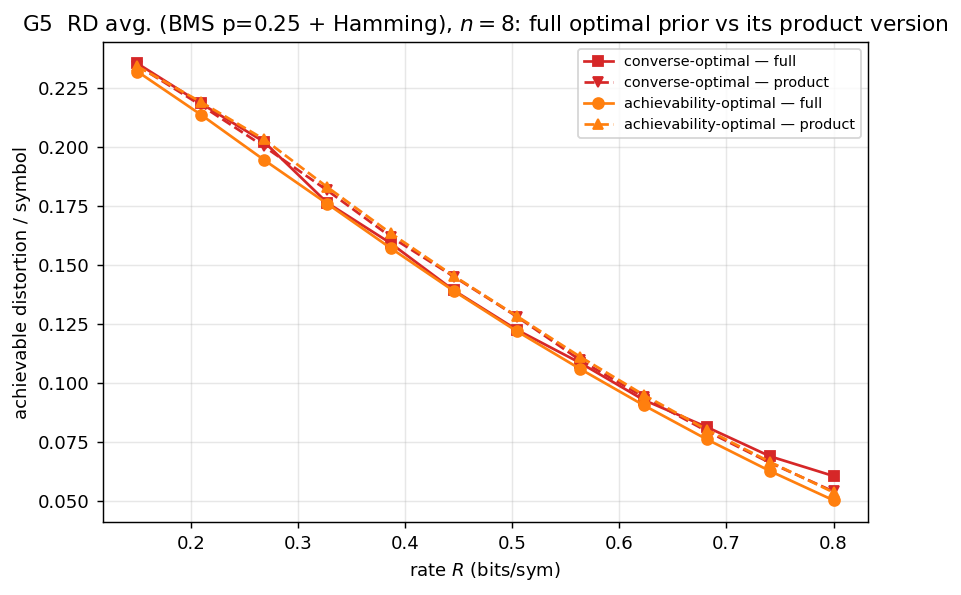
\includegraphics[width=\linewidth]{rd_avg_g5_full_vs_product_n8.png}\caption{$n=8$}\end{subfigure}\hfill
\begin{subfigure}{0.49\textwidth}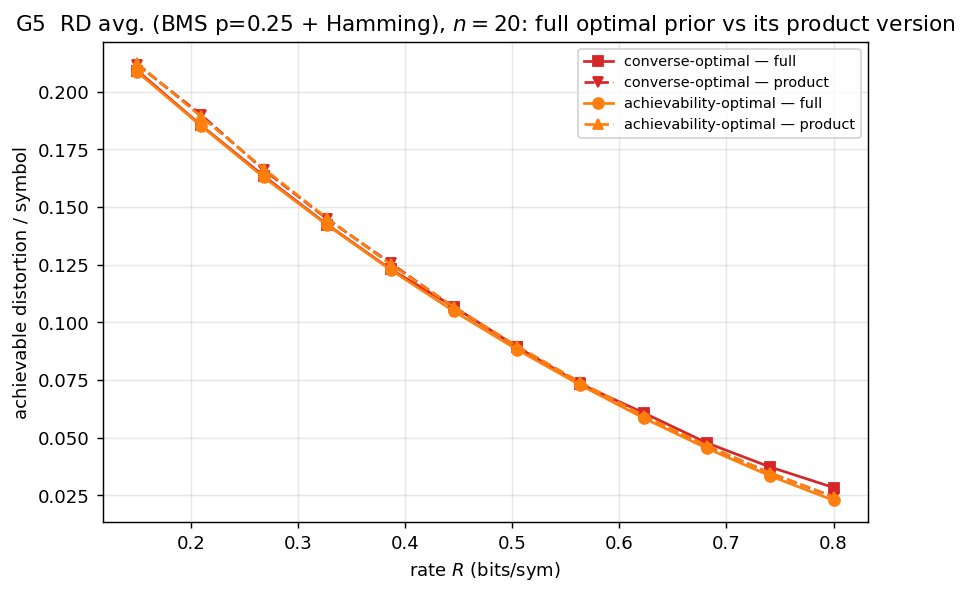
\includegraphics[width=\linewidth]{rd_avg_g5_full_vs_product_n20.png}\caption{$n=20$}\end{subfigure}
\caption{G5 --- full vs.\ product prior. All four curves coincide: average
distortion is prior-insensitive.}
\end{figure}

\subsection{Rate--distortion, excess --- BMS$(0.25)$, $T=1$, $n=6$}
Excess distortion is the best-of-$M$ of the block indicator, a lifted quantity, so
$n=6$. The gain peaks at $\approx7\%$; reusing the converse prior costs $2.8\times$
($P_{\mathrm{exc}}:4.5\mathrm{e}{-}2$ vs.\ $1.6\mathrm{e}{-}2$).
\begin{figure}[H]\centering
\begin{subfigure}{0.49\textwidth}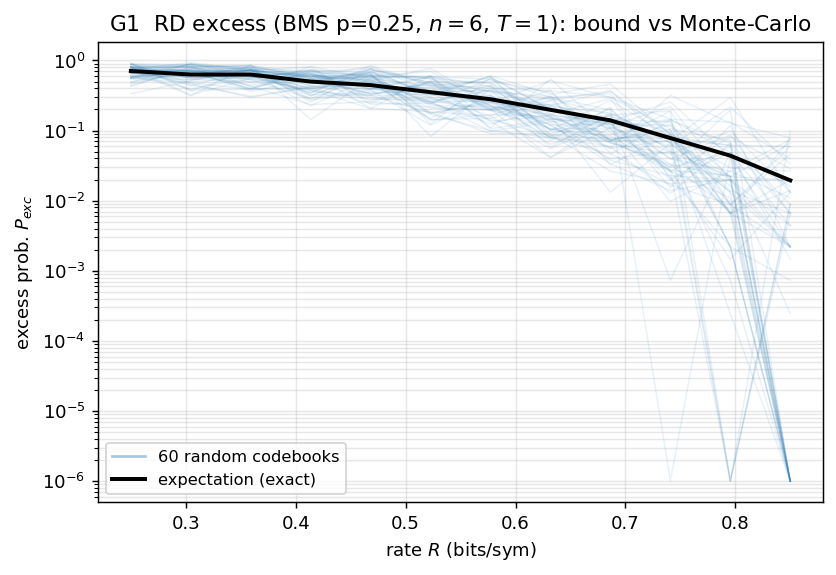
\includegraphics[width=\linewidth]{rd_exc_g1_mc_spread.png}\caption{G1}\end{subfigure}\hfill
\begin{subfigure}{0.49\textwidth}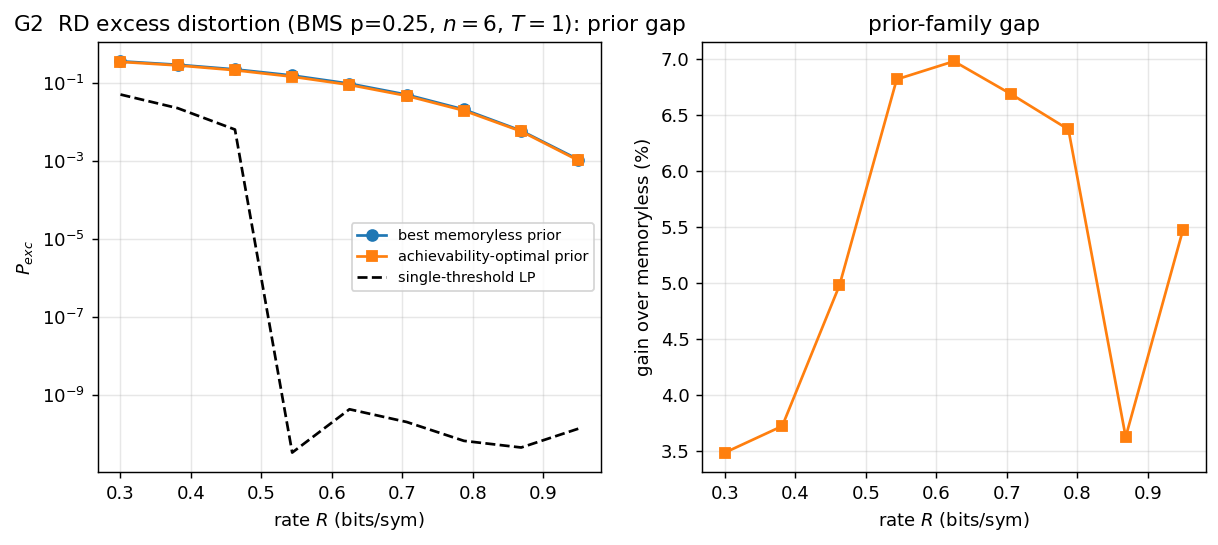
\includegraphics[width=\linewidth]{rd_exc_g2_prior_gap.png}\caption{G2}\end{subfigure}
\\[4pt]
\begin{subfigure}{0.49\textwidth}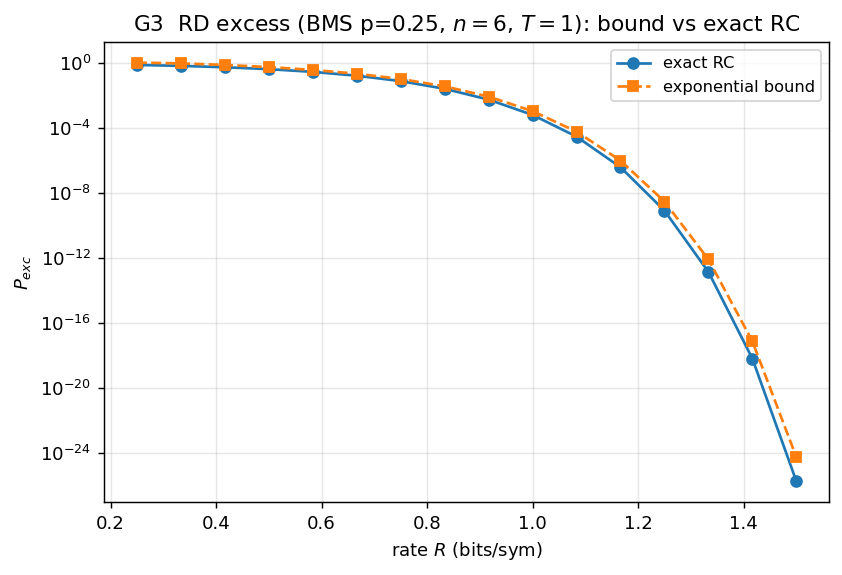
\includegraphics[width=\linewidth]{rd_exc_g3_bounds_vs_exact.png}\caption{G3}\end{subfigure}\hfill
\begin{subfigure}{0.49\textwidth}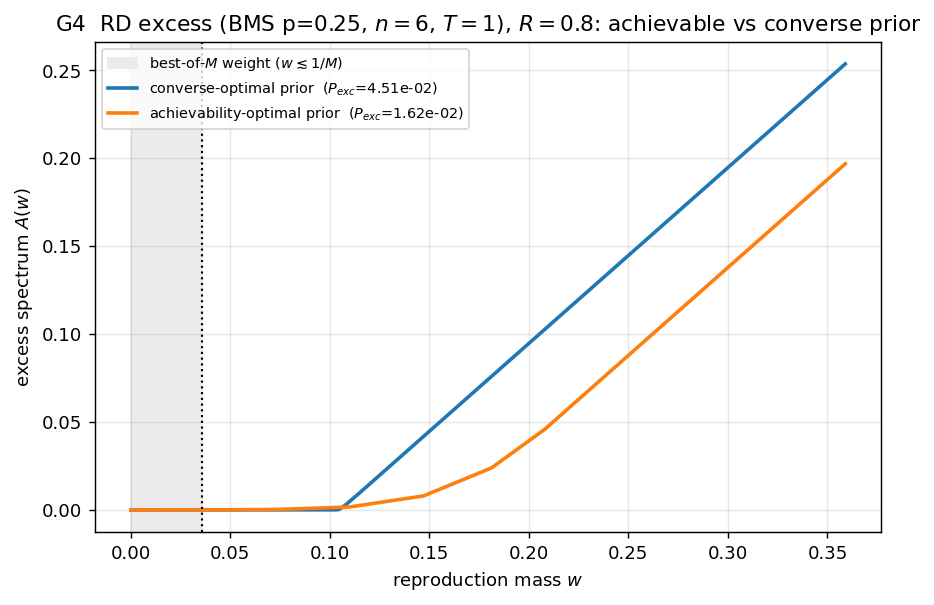
\includegraphics[width=\linewidth]{rd_exc_g4_fcurve_compare.png}\caption{G4}\end{subfigure}
\caption{Excess distortion: bound vs.\ MC (G1), prior gap (G2), exact vs.\ bound
(G3), and the excess spectra (G4); the converse-marginal prior is the worst here.}
\end{figure}
\begin{figure}[H]\centering
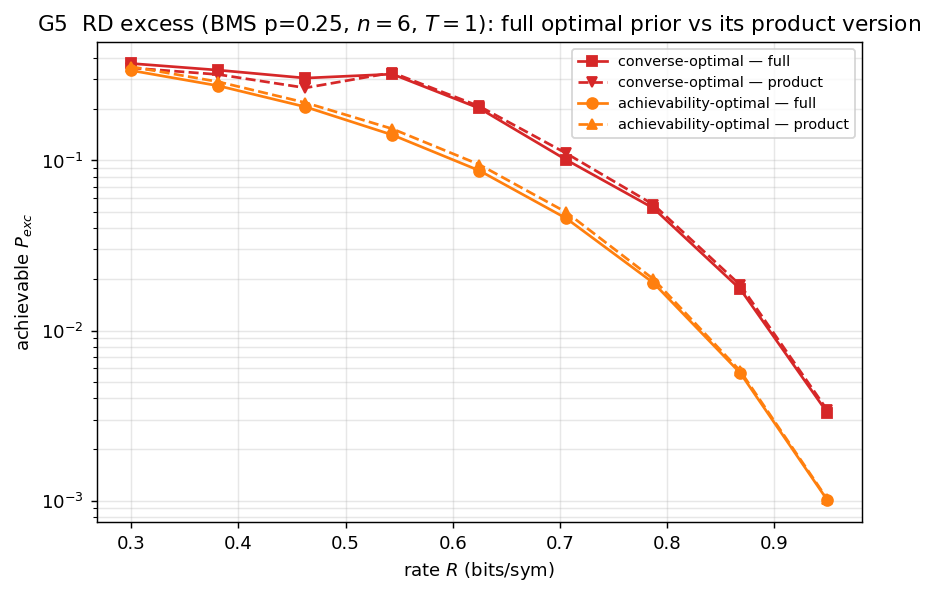
\includegraphics[width=0.62\textwidth]{rd_exc_g5_full_vs_product.png}
\caption{G5 --- full vs.\ product prior. The converse pair sits $\approx2.8\times$
above the achievable pair, and---unlike channel coding---marginalizing the converse
prior does \emph{not} rescue it (full and product overlap).}
\end{figure}

\subsection{JSCC --- BMS$(0.07)$ over BSC$(0.05)$, $H<C$}
With $H=0.366<C=0.714$ bit the source is transmissible. The coded bounds (converse,
and the $\mathrm{RCU}^+$ achievable bound at the march optimum) fall with $n$, while
the uncoded symbol-by-symbol scheme degrades; they cross near $n\approx4$.
\begin{figure}[H]\centering
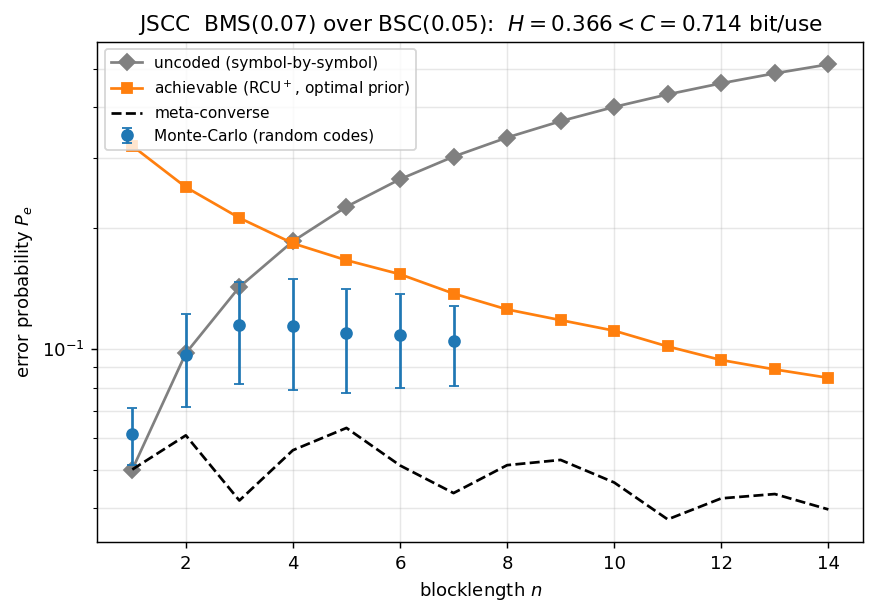
\includegraphics[width=0.72\textwidth]{jscc_error_vs_n.png}
\caption{JSCC error probability vs.\ blocklength: meta-converse, achievable
($\mathrm{RCU}^+$ via the simplex march), Monte-Carlo of random codes, and the
uncoded baseline.}
\end{figure}

\section{Conclusion}
Prior optimization of the achievability bound is one convex program
$\max_Q c\Tr\Phi(AQ)$; the kernel chooses $\Phi$, and a single first-order simplex
march---KKT-certified, exact for any kernel---solves it across channel coding,
rate--distortion, and JSCC. With the certified optimum in hand the headline finding
is rigorous rather than heuristic: for these minimal settings the memoryless prior
is within a few percent of optimal, while the \emph{converse} prior, reused for
achievability, can be far from it.

\end{document}
